\chapter{Blockchain technology} \label{chap:Blockchain}

As identified in the introduction, blockchain is difficult for many to understand as it lies at the intersection of cryptography, game theory, computer networking, data transmission and monetary theory.\footcite[Cf.][]{LoppNobodyUnderstandsBitcoin2017} The different concepts interact very closely and thus multiple elements must be understood concurrently.\footcite[Cf.][p.2]{SwellerVisualisationInstructionalDesign2002} This chapter gives a  brief introduction to the technology. It provides an overview of the motivation behind its creation and the general elements of a blockchain, and subsequently examines possible application fields of the technology. 
% Wieso ist Blockchain für viele so schwer zu verstehen? -> Intersection of different topics -> Information Structures (Sweller 1994)

\section{An overview of blockchain technology} \label{sec:Blockchain}

Blockchain technology was first introduced in the wake of the global economic crisis in 2008, when a person under the pen name Satoshi Nakamoto presented a concept for a new digital currency.\footcite[Cf.][]{Nakamoto.2008} Nakamoto introduced the digital currency bitcoin with the motivation to provide a financial system without relying on banks or other financial institutions as intermediaries. In his paper, Nakamoto criticizes the central role of the financial institution controlling digital transactions between two parties and forcing these two parties to trust the institution. He, therefore, developed a system allowing any two parties to conduct transactions directly with each other, thus removing the need for a trusted third party.\footcite[Cf.][p.2]{Nakamoto.2008} A blockchain can be thought of as a decentralized ledger which records the entire transaction history. A transaction refers to one change made in the ledger (e.g., the payment of one bitcoin from A to B). The name blockchain stems from the fact that transactions are bundled into blocks. Each block in the blockchain (except for the first, i.e., genesis block) references a previous block.\footcite[Cf.][chapter 1]{BashirMasteringBlockchain2017} This reference takes place in form of hash values.\footcite[Cf.][p.351]{AntonopolousAndreasM..2017} The hashing algorithm is a mathematical one-way function which maps a block as an input to a fixed-length deterministic output producing a digital fingerprint of the block.\footnote{For any specific input, the resulting hash will always be the same and can be easily calculated and verified by anyone implementing the same hash algorithm.} By connecting the blocks via their hashes, all changes in the ledger can be reconstructed and all transactions are at all times visible. The blockchain runs on a peer-to-peer network of computers provided by volunteers around the world. Each node participating in the network has its own copy of the blockchain, hence giving all nodes the same view of the blockchain.\footcites[Cf.][p.5]{Tapscott.2017}[cf.][p.41]{Welzel.2017} Its distributed nature allows the system to stay healthy even if some nodes quit the network or are compromised. This approach protects the blockchain against possible power outages or unilateral manipulation.\footcite[Cf.][p.8]{Nakamoto.2008}

To establish a consensus between the nodes regarding agreement on which transactions are valid and can be included in the blocks, the participating nodes first check the validity of every new transaction. This is done by cryptographically verifying that the initiating party actually owns the coins it is sending and that the coins have not been spent on something else.\footcite[Cf.][p.68]{AntonopolousAndreasM..2017} Then, the nodes participate in a distributed consensus mechanism to build the next block that is then appended to the blockchain. In the case of bitcoin, this takes place on the basis of the proof of work algorithm.\footcites[Cf.][]{Dwork.1993}[cf.][p.3]{Nakamoto.2008} Proof of work takes advantage of a cryptographic puzzle, where a node has to use its computing resources in order to find a random number, called nonce (number used only once), so that the hash of the signature of the previous block, the transactions of the current block, a time stamp, and said nonce results in a value that has a specific set of leading zeroes. The cryptographic puzzle is secured against cheating because two similar values result in two totally different and random hashed values. It is not possible with today's tools to calculate the original value from a hashed value.\footcite[Cf.][p.12]{SwanBlockchainblueprintnew2015} This cryptographic puzzle therefore forces the node to use its CPU capacity to find a random nonce. Only with such a nonce will a new block broadcast to the network be accepted by the other nodes.\footcites[Cf.][p.8]{Nakamoto.2008}[cf.][p.12]{Schutte.2017} Apart from the CPU based proof of work algorithm, there are a number of other distributed consensus mechanisms. For example, the proof of work approach has been adapted to a memory based algorithm where the puzzle has to be solved by a specific number of memory reads.\footcite[Cf.][]{Abadi.2005} It has also been adapted to a network-based approach where the puzzle is solved by communicating with other nodes on the network and using their information to complete the puzzle.\footcite[Cf.][]{Abliz.2009} Another approach is proof of stake, which another blockchain implementation (Ethereum) is planning to apply. In this approach, the nodes that can \enquote{stake}\footnote{\textit{Staking a  new block} is the term used for creating a new block to append to the blockchain in a proof of stake system. This is analogous to the term \textit{Mining a new block} which is used in proof of work systems.} a new block are chosen by their staked share of their digital currency\footcite[Cf.][]{King.2012} or they are chosen randomly.\footcites[Cf.][]{w.A..2016}[cf.][p.200]{AntonopolousAndreasM..2017}[cf.][p.11 et seq]{Schlatt.2016} Two variants of the proof of stake consensus mechanism exist: delegated proof of stake and leased proof of stake. Delegated proof of stake extends the consensus mechanism by incentivizing participants with lower balances (which in the traditional proof of stake implementation would be unlikely to stake a block) to use their balance to elect a list of nodes which would have the opportunity to stake a block. Or, with leased proof of stake, the nodes with low balances may lend their coins to staking nodes (which would then be more likely to stake a new block) and they receive a share of the staking node's reward in return.\footcites[Cf.][p.12]{CataliniSimpleEconomicsBlockchain2017}[cf.][p.5 et seqq]{DavidsonEconomicsBlockchain2016}   

% Independently of its consensus mechanism, a blockchain can take different forms:\footcite[Cf.][p.10-12]{Schlatt.2016}
% \begin{itemize}
%   \item \textbf{Public Blockchain:} The ledger is public and everyone can join the network.
%   \item \textbf{Private Blockchain:} The ledger is accessible to a predefined set of users.
%   \item \textbf{Permissionless Blockchain:} All nodes in the network are equal and all can append to the blockchain.
%  \item \textbf{Permissioned Blockchain:} A predefined subset of nodes in the network has the right to append to the blockchain. All nodes broadcast their transactions to the network but only the permissioned nodes create new blocks.
% \end{itemize} 

% \begin{figure}[h]
%  \centering
%  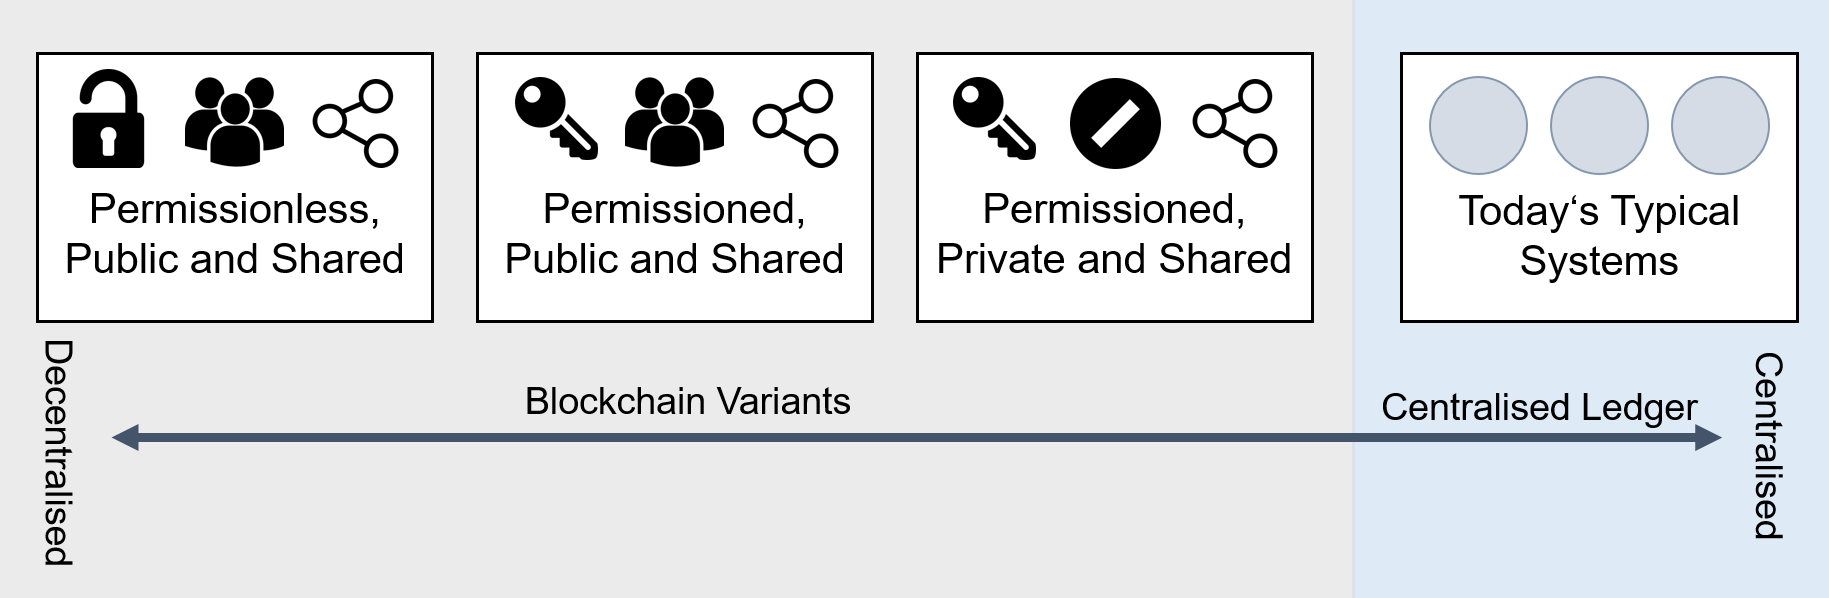
\includegraphics[width = \textwidth]{graphics/Picture1.png}
%  \caption{Different blockchains vary in their degree of centralization, adapted from \cite{GOV.2016}.}
%  \label{fig:DLTs}
% \end{figure}

The capabilities of blockchain go far beyond providing a distributed ledger if smart contracts are used. Smart contracts are pieces of code in a transaction which are executed when nodes validate that transaction. These smart contracts extend the capabilities of blockchain to allow trusted and automatic modification of information.\footcite[Cf.][p.14]{Schutte.2017} They are in their essence a digital copy of a conventional contract, defining the rules and punishments in the case of non-compliance in lines of code. The concept of describing a contract with code was introduced in 1997 by Nick Szabo\footcite[][]{Szabo.1997} but only in combination with blockchain can it be implemented to develop its full potential.\footcites[Cf.][p.23]{Schlatt.2016}[cf.][p.22-24]{GOV.2016} Processes, which validate the integrity of an entity, may be fully automated by using blockchain technology and smart contracts.

Blockchain technology shows the following characteristics: It is distributed, digital transactions no longer necessitate a middleman to be executed securely. The blockchain is encrypted, using public and private key pairs to establish virtual security. Blockchain is public, anyone is able to view all transactions at all times because they lie on the network and not in one central database, and the code is open-sourced. Finally, the technology enables an immutable, complete history of all transactions.\footcite[Cf.][p.5]{Tapscott.2017} All these characteristics combined constitute blockchain's potential to disrupt economic sectors by providing a new way to securely store valuable digital assets and to transact between untrusted parties. They rely on the interplay of different underlying concepts, which the next paragraph summarizes under the term cryptoeconomics.

\paragraph{The cryptoeconomics of blockchain} From another point of view, blockchain may also be described as the product of financial, economic and \ac{IT} concepts. In this paper, cryptoeconomics refers to these three underlying concepts,\footnote{Cf. \cite{BabbittCryptoeconomicDesignProposed2015}, p.1. Note, that different definitions of this term exist due to its very young age.}  which have existed long before the advent of blockchain, but were previously regarded independently from each other.\footcites[Cf.][p.2]{DavidsonEconomicsBlockchain2016}[cf.][p.21]{AntonopolousAndreasM..2017}[cf.][p.110]{RabahDigitalCryptoeconomicsPowered2017}
\begin{itemize}[noitemsep]
    \item \textbf{\ac{IT}}: The above-described characteristics are enabled by the combination of cryptography (public and private key infrastructure, elliptic curve cryptography, hash functions) and distributed systems (peer to peer network, concurrency, append-only data structures).
    \item \textbf{Finance}: While the concepts within \ac{IT} describe a logical world within the realms of mathematics, the introduction of humans necessitates the consideration of further concepts such as monetary theory regarding the question \enquote{What is money?} and the intrinsic value of goods.
    \item \textbf{Economics}: It also requires the consideration and application of economic values and game-theoretic approaches, such as the role of markets, definition of supply \& demand, the incentivization of market players, resulting in the development of the presented consensus mechanisms, and thus, the generation of valuable digital assets.\footcite[Cf.][\textit{Cryptoeconomics}]{BashirMasteringBlockchainSecond2018}
\end{itemize}

% \section{Transactions} \label{sec:TX}

% Inspect transactions in detail, show how they are broadcast and put into blocks
% -> only in ethereum or bitcoin or should I inspect the overall design of transaction by looking at different coins?

% Even though the first implementation of blockchain was motivated by providing a decentralized alternative to financial institutions,\footcite[Cf.][p.2]{Nakamoto.2008} the new defined data structure offers a variety of additional use cases that will be explored in the following section.

\section{Applications of blockchain technology} \label{sec:SmartContracts}
The growing interest in the blockchain technology, mostly driven by the rise in popularity of the cryptocurrency bitcoin, has revealed that the technology covers various use cases which are explored in the following paragraphs. The applications of the technology are multi-faceted and too numerous to be listed in their entirety in this section. For more detailed information about possible applications, please refer to \cite{AntonopolousAndreasM..2017}, \cite{SchatskybitcoinBlockchaincoming2015}, or \cite{Schutte.2017}.

Blockchain is best used in the case of a shared repository of information that multiple parties access. These parties all generate information in the form of transactions requiring modifications to the state of the shared repository. For the blockchain to be really effective, the parties creating these transactions should mistrust each other to a certain degree. In addition, smart contracts then allow the automatic modification of the information in the repository and may create dependencies between transactions, thus also enabling the representation of business processes.\footcites[Cf.][p.8]{MulliganBlockchainHypePractical2018}[cf.][p.5]{Tapscott.2017}[cf.][p.166]{DannenIntroducingethereumsolidity2017}

An example for this in the financial sector is the near real-time settlement of cross-border payments or securities trading between institutions.\footcite[Cf.][]{SchatskybitcoinBlockchaincoming2015} Another example would be the exchange of sensitive medical records between health institutions, doctors, and patients where the patients may keep ownership over their data and determine who accesses their data.\footcites[Cf.][p.170]{DannenIntroducingethereumsolidity2017}[cf.][p.18]{Schutte.2017} This may also apply to the public sector, maintaining registers and certifications that require an especially high degree of trust – such as a commercial register or a land register. Blockchain may also enable tamper-proof electronic elections or ensure efficient data exchange between authorities where the citizen may remain in control of their data at any time and, for example, grant access to authorizations which is limited in time and content.\footcites[Cf.][p.18]{Schutte.2017}  

% A similar concept may be used for social networks where the user may keep ownership over their data, allow specific services to access their personal information, and where they may be incentivized to publish content or to interact with the network in the form of micropayments (very small, yet feasibly payments of ,e.g., 1 cent).

Blockchain also proves useful for other industries, such as consumer products and retail, where companies can track their assets and use that information to improve their supply chain processes or warranties.\footcite[Cf.][p.31]{GOV.2016} An example in the automotive industry might be the tracking of a car's mileage to ensure it is not tampered with. Sensors could read the car's mileage, send it to a shared repository, which the car manufacturer and the car owner may access to have access to trustworthy data. %This would benefit both the consumer and the producer as they may base their buying decision (or any decisions regarding warranty claims) on trustworthy data. In addition, it would also be possible to allow an insurance company to access this data.

Although this is only a very limited description of use cases, the selection illustrates that blockchain provides a myriad of possible application scenarios. However, due to its emerging nature and high complexity, it does not always offer the ideal solution to a problem. This is especially the case when the problem does not necessitate a distributed solution, as in many instances a database might suffice.\footcites[Cf.][P152, P154]{BerndKammholz_Interview}[cf.][P23]{DanielKaltenbach_Interview} The importance here is, therefore, to educate professionals about the ideal application scenarios, so that they may identify themselves whether they actually need blockchain or not.
